We use hashing in the dictionary problem.
A dictionary is a collection of objects: $D = \{O_1, O_2, \_, O_n\} \subseteq U$ composed by $<key, satellite\_data>$.
Over this collection we want:
\begin{itemize}
    \item $search(k)$ to check if $k \in D$;
    \item $insert(O)$;
    \item $delete(k)$.
\end{itemize}

NB: search is exact search, so if we search for $x$ we are looking for an exact match, not a prefix, not search with error.
It's also called \emph{membership query}.

\section{Hash function}
We define an hash function as:
$$
    h : U \xrightarrow{} [m]
$$
with $[m] = \{0, 1, \_, m-1 \}$ with $m << |U|$.
So $h$ takes $log_2 |U|$ bits and returns $log_2 m$ bits, and the result is called a fingerprint or a digest, that's why we impose $m,n << |U|$.

NB: if $U$ is small there is no need for hash table, we can just use a Direct Access Table which is a table with the same key as the index.

\section{Classic approaches}
\subsection{Hashing with chaining}
We use an array of size $m$ and each cell is a pointer to a linked list, each list contains some entries of the hash table.
Whenever we want to add an object we get it's digest and use it to index the array, then we add the entry to the corresponding linked list.
The search is of course just a lookup for the digest and a list traversal, deletion is a search and a deletion in the linked list.
Basically we use a direct access table and use a linked list to deal with the hash collisions.
\begin{figure}[H]
    \centering
    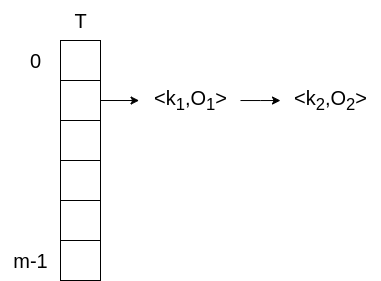
\includegraphics[width=200px]{images/7_Hashing/chained_hashing.png}
\end{figure}
The total space is then $O(m+n)$ plus of course the satellite data, so in a more formal way:
$$
    m \cdot log_2 m + n \cdot [L + 2 \cdot 64] + \text{satellite data}
$$
in which $log_2 m$ is the size of a pointer to an item, $L$ is the size of a key and $2 \cdot 64$ is the size of the forward and backward pointer of the linked list.

We want to upper bound the access time, so we need something to estimate the number of elements inside each list, let's use the assumption of \emph{simple uniform hash}:
$$
    \mathbb{P}(h(k) = i) = \frac{1}{m}
$$
so:
$$
    \mathbb{E}[search] = 1 + \mathbb{E}[len(list)] = 1 + \sum_{k \in D} 1 \cdot \mathbb{P}(h(k) = i) = 1 + \sum_{k \in D} 1 \cdot \frac{1}{m} = \frac{n}{m}
$$
We will call $\alpha = \frac{n}{m}$ the \emph{loading factor} of the hash table.

\subsection{Global rebuilding technique}
Another approach which exploits the \emph{amortised argument} states that after some insertions we need to rebuild the entire table, for example:
\begin{itemize}
    \item we start with $n = n_0$ elements, so we create an hash table with $m_0 = 2 \cdot n_0$ as a size;
    \item we then have some insertions;
    \item whenever we hit $n = 2 \cdot n_0$ we rebuild the entire table with $m_1 = 4 \cdot n_0$.
\end{itemize}
Of course if we delete enough item we rebuild the table, too in order to reduce the memory consumption!

Let's estimate the cost of an insertion between the two builds:
$$
    1 + \frac{n}{m_0} = 1 + \frac{n}{2 \cdot n_0} \leq 1 + \frac{n_0}{2 \cdot n_0} = 1 + \frac{1}{2} = O(1)
$$
so the total cost of inserting phase is $\Theta(n_0)$.
Since we've paid $\Theta(n_0)$ to execute $n_0$ operations we can state that the amortized cost of each insertion is:
$$
    \frac{\Theta(n_0)}{n_0} = \Theta(1)
$$

\subsection{Problem of simple uniform hashing}
In order to be \emph{simple uniform hash} we need that $ \exists h \in \mathbb{H}$ such that it can map every key in $U$ in every slot of the hash table.

Let's compute the possible number of mappings to count how many functions corresponds to the definition:
\begin{itemize}
    \item for $k_1$ we need to have a mapping for 0, 1, 2, \_, $m-1$;
    \item for $k_2$ we need to have a mapping for 0, 1, 2, \_, $m-1$;
    \item \_
    \item for $k_U$ we need to have a mapping for 0, 1, 2, \_, $m-1$.
\end{itemize}
Reducing to 2 keys we have $m^2$ mappings, enlarging to $U$ keys we have $m^U$ mappings, let's call that set $\mathbb{H}$.
In order to represent each $h \in \mathbb{H}$ we need $\geq log_s m^U = U \cdot log_2 m$ bits, which is impossible in computational terms!

\section{Universal hashing}
We define the universal hashing as:
$$
    \mathbb{H} = \{ h : U \xrightarrow{} [m] : \forall x, y \in U, x \neq y : \#H[h(x) = h(y)] \leq \frac{\mathbb{H}}{m} \}
$$
so: fixed a pair of different keys $<x, y>$ the number of functions for which there is a collsion is a fraction of $\mathbb{H}$.

Assuming that hypothesis the probability of picking a function for which there is a collision is:
$$
    \frac{\frac{|\mathbb{H}|}{m}}{|\mathbb{H}|} = \frac{1}{m}
$$

\subsection{Cost of hashing with chaining and universal hashing}
$$
    \mathbb{E}[len(list)] = \sum_{k' \in D} 1 \cdot \mathbb{P}(h(k) = h(k')) = \sum_{k' \in D} \frac{1}{m} = \frac{|D|}{m} = \frac{n}{m} = \alpha
$$
with $h$ chosen at random, we have the same result as before but with a better property since can be effectively used.

\subsection{Example of universal hashing, with proof}
We want to build $h_a : U \xrightarrow{} [m]$ with $a \neq 0$ and $m$ prime.
To do it we start from a generic key $k \in U$ and we split it in $r$ blocks such that each block is of size $log_2 m$ bits so:
$$
    r = \frac{log_2 |U|}{log_2 m}
$$
We choose $a \in U$ at random but $a \neq 0$ so:
$$
    \mathbb{H} = \# a \text{ with } a \neq 0 = |U| - 1
$$
and we split it in $r$ blocks too.
Then we define:
$$
    h_a(k) = \sum_{i = 0}^{r-1} a_i \cdot k_i \mod m
$$
That can be seen as scalar product between two vectors.

\subsubsection{Proof of universal hashing}
Let's fix $x \neq y \in U$ we want to show that:
$$
    \#h_a : [h_a(x) = h_a(y)] \leq \frac{|\mathbb{H}|}{m}
$$
which is equivalent to the universal hashing function.

Let's estimate the $\#a$ such that:
$$
    \sum_{i = 0}^{r-1} a_i \cdot x_i = \sum_{i=0}^{r-1} a_i \cdot y_i \mod m
$$
since $x \neq y$ at least a block of $x$ and $y$ is different, let's suppose that the different blocks are $x_0$ and $y_0$:
$$
    a_0 \cdot (x_0 - y_0) = - \sum_{i=1}^{r-1} a_i \cdot (x_i - y_i) \mod m
$$
since $x_0 - y_0$ is not zero and we have a prime modulus there exists an inverse for it:
$$
    a_0 = - (x_0 - y_0)^{-1} \sum_{i=1}^{r-1} a_i \cdot (x_i - y_i) \mod m
$$
so in order to have a collision $a_0$ must be chosen according to the relation above, but of course $a_1, \_, a_{r-1}$ are free to be choosen.

So the values of $a$ are the different ways we can choose $a_1, \_, a_{r-1}$ which is $m^{r-1} -1$ (-1 because we don't count the 0 combination) so:
$$
    m^{r-1} -1 = \frac{m^r}{m} - 1 = \frac{|U|}{m} - 1 \leq \frac{|U| - 1}{m} = \frac{|\mathbb{H}|}{m}
$$

NB: of course the usage of $m$ prime is not so good for our uses, we would like to have something in the form of $2^x$ because we want fast operations like shift and bitmasks, so we can use:
$$
    h_a(k) = \left[ \sum_{i=0}^{r-1} a_i \cdot k_i \mod p \right] \mod m
$$
with $p$ the prime number and $m$ a power of 2.

\subsection{Another universal hashing}
We would like to save computational speed avoiding multiplication and divisions.
Let's assume $|U| = 2^q$, $m = 2^l$, $a$ odd, we define:
$$
    \mathbb{H}_{q,l} = \{ h_a(x) = (a x \mod 2^q) div 2^{q-l} \}
$$
$a$ and $2^q$ are coprime, so we have a shuffling.
Since $|a| = log_2 |U|$ and $|x|=log_2 |U|$ then $|a \cdot x| = 2 log_2 |U|$, we take the last $log_2 |U|$ bits of $a \cdot x$, then $q = log_2 |U|$ and $l = log_2 m$ so in the end we got the upper part of $a \cdot x \mod 2^q$:
\begin{figure}[H]
    \centering
    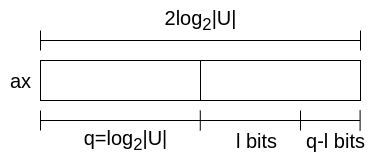
\includegraphics[width=200px]{images/7_Hashing/another_universal_hash.png}
\end{figure}
So basically we compute a multiplication and keep the middle bits.

\section{d-left hashing}
It's used to remove the number of pointers in order to save space.
We start from a table of size $m$ and split it into bins of $b$ slots, so we have $\frac{m}{b}$ bins.
We use $d$ different hashing functions and for each key we compute $d$ hashes, access those bins and we place the element inside the most empty to store the object!

Search is constant because we compute hashes and scan the bins:
$$
    \mathbb{E}[\text{length of the longest list}] = \frac{log_2 log_2 n}{log_2 d} + O(1)
$$
when $d \geq 2$.

So if we increase the number of hashing functions we improve the length of bins by very little (it's logarithm factor) but the time complexity increases linearly so the best choice is when $d = 2$.

\subsection{Power of two choices}
It's important to note that in $d=1$, which is basically the hash with chaining we have:
$$
    \mathbb{E}[\text{length of the longest list}] = \frac{log_2 n}{log_2 log_2 n}
$$
so moving from $d=1$ to $d=2$ we have an exponential improvement in length of lists.

\section{Cuckoo hashing}
It's a sort of perfect hashing because provides us:
\begin{itemize}
    \item search in $O(1)$ worst case;
    \item deletion in $O(1)$ worst case;
    \item insertion in $O(1)$ amortized expected time (which means that on average the cost is spread among different insertions).
\end{itemize}

We start from an array of $m$ cells with $m \geq n$, we use two hash functions $h_1$ and $h_2$ to access table to check the bins:
\begin{itemize}
    \item if one of them is empty we put the value inside it;
    \item if both are filled we put the key into one of them and we relocate the key we've removed:
    \begin{figure}[H]
        \centering
        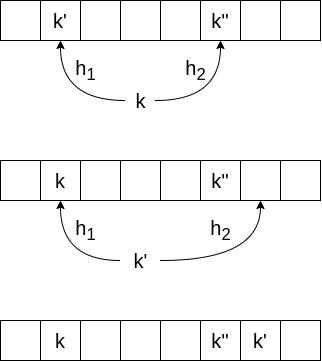
\includegraphics[width=150px]{images/7_Hashing/cuckoo_relocation.png}
    \end{figure}
\end{itemize}

\subsection{Theorem 1}
$$
    \forall i, j, \forall c > 1, m \geq 2 c n \implies \mathbb{P}(\text{shortest path from i to j is of length L}) \leq \frac{1}{mc^L}
$$
We use the concept of path because we can see the cells as nodes of a graph and as arcs we connect the two nodes that can be reached from the key $k$, so:
\begin{itemize}
    \item $\#$nodes = $m$ = $\#$cells;
    \item $\#$edges = $n$ = $\#$keys.
\end{itemize}
path is important because it states how many jumps we can do during relocations.

It's important to notice that:
$$
    \alpha = \frac{n}{m} \leq \frac{\frac{m}{2c}}{m} = \frac{1}{2c} < \frac{1}{2}
$$
so it means that the hash table is half filled which is not so good for space occupancy.
Let's prove the theorem in that case by induction on $L$:
\begin{itemize}
    \item $L=1$:
    $$
        \mathbb{P}(\text{shortest path from i to j is of length 1}) = \mathbb{P}(\text{there is an edge from i to j}) = 
    $$
    $$
        = \mathbb{P}(\exists k : (h_1(k) = i \land h_2(k) = j) \lor (h_1(k) = j \land h_2(k) = i) ) 
    $$
    applying the union bound:
    $$
        \leq \sum_{k \in D} \frac{2}{m^2} = \frac{2n}{m^2}
    $$
    $m \geq 2cn \implies 2n \leq \frac{m}{c}$:
    $$
        \leq \frac{\frac{m}{c}}{m^2} = \frac{1}{cm}
    $$

    \item assuming that for $L-1$ is true let's prove it for $L$:
    $$
        \mathbb{P}(\text{shortest path from i to j is of length }L)
    $$
    $$
        = \mathbb{P}(\exists \text{path of length $L-1$ from i to z} \land \text{path from $z$ to $j$ of length 1})
    $$
    applying the union bound:
    $$
        \leq \sum_z \mathbb{P}(\text{there is a path from i to z of length $L-1$} \land \text{ there is an edge from z to j})
    $$
    applying the inductive hypothesis:
    $$
        = \sum_z \frac{1}{mc^{L-1}} \cdot \frac{1}{mc} = \sum_z \frac{1}{m^2 \cdot c^L} = m \cdot \frac{1}{m^2 \cdot c^L} = \frac{1}{m \cdot c^L}
    $$
\end{itemize}

\subsection{When cuckoo hashing fails}
Let's use $h_1(x) = x \mod 7$, $h_2(x) = 2x \mod 7$, $m = 7$ and let's insert 1, 3, 8, 15:
\begin{itemize}
    \item 1 can go both into $h_1(1) = 1$ and $h_2(1) = 2$, we insert it into 1;
    \item 3 can go both into $h_1(3) = 3$ and $h_2(3) = 6$, we insert it into 3;
    \item 8 can only go into $h_2(8) = 2$ since $h_1(8) = 1$ is already filled;
    \item 15 neither can go into $h_1(15) = 1$, nor $h_2(15) = 2$, so we need to relocate something, let's check the graph;
    \begin{figure}[H]
        \centering
        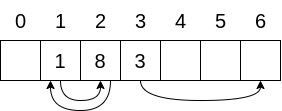
\includegraphics[width=150px]{images/7_Hashing/cuckoo_hashing_cycle.png}
    \end{figure}
    we have a cycle between 1 and 2 and we want to insert something in one of the two, so the insertion fails!
\end{itemize}

NB: just one cycle is not enough to fail an insertion, what we need for failing is two cycles and an insertion which joins them!

\subsection{Failing}
$$
    \mathbb{P}(failing) \leq \mathbb{P}(\text{exists 2 cycles}) \leq \mathbb{P}(\exists \text{cycles}) =
$$
$$
    \mathbb{P}(\exists z, L: \text{there is a path from z to z of length L})
$$
applying union bound:
$$
    \leq \sum_{z \in T} \sum_{L \geq 1} \frac{1}{mc^L} = \sum_{z \in T} \frac{1}{m} \sum_{L \geq 1} \left( \frac{1}{c} \right)^L
$$
since $c > 1$ it's a known series:
$$
    = \sum_{z \in T} \frac{1}{m} \cdot \frac{1}{c-1} = \frac{1}{c-1}
$$

\subsection{Amortized cost in insertion}
Fixing $c=3$ we have:
$$
    \mathbb{P}(\text{insertion will fail}) \leq \frac{1}{2}
$$
$$
    m \geq 6n \implies \alpha = \frac{n}{m} \leq \frac{1}{6}
$$
which are not so nice.

So we have a huge table and half of insertions will fail, but let's check the amortized expected cost:
\begin{itemize}
    \item we start supposing of having $n_0 + \epsilon n_0$ keys, so we will build a table with $m_0 = 6(1 + \epsilon)n_0$ but having only $n_0$ actual keys;
    \item after $\epsilon n_0$ insertions we have filled the available space so $m_0 = 6 \cdot \#$keys.
\end{itemize}
Since $m \geq 6n$ the probability of insertion fails is $\leq \frac{1}{2}$.

We sit at the end of the insertions and asks us the probability of failing over the past $(1 + \epsilon)n_0$ insertions, it's $\frac{1}{2}$ so we do at most 2 constructions before achieving that amount of insertions (which means we redraw $h_1$ and $h_2$).

Since construction cost is linear if we distribute it over all the $n_0$ insertions we have amortized cost.
So:
$$
    \text{if } c \leq 2, \forall x, y \mathbb{P}(\text{there is a path from x to y}) = \frac{1}{m}
$$
which means that $x$ and $y$ collides:
$$
    = \mathbb{P}(\exists L : \text{exists a path of length L from x to y})
$$
applying the union bound:
$$
    \leq \sum_{L \geq 1} \frac{1}{mc^L} = \frac{1}{m} \sum_{L \geq 1} \frac{1}{c^L}
$$
since $c > 1$ it's a known series:
$$
    = \frac{1}{m} \cdot \frac{1}{c-1}
$$
for $c = 2$ it's $\frac{1}{m}$ and for $c > 2$ it's $\leq \frac{1}{m}$, so:
$$
    \mathbb{P}(collision) \leq \frac{1}{m}
$$

So average \#keys colliding with some keys $k$ is $\frac{n}{m} \leq 1$, so the average insertion cost is $O(1)$ time expected.

But the space occupancy continues to be bad!
\subsubsection{In practice}
In practice we mix d-left and cuckoo hashing so instead of single cells we use buckets.
It guarantees 95\% of occupancy!

\section{Minimal Ordered Perfect Hash Function}
\subsection{Perfect hash function}
$h$ is a perfect hash iff:
$$
    \forall k_1, k_2 \in D, k_1 \neq k_2 \implies h(k_1) \neq h(k_2)
$$
basically: no collisions among the elements in the dictionary.
That's useful because it guarantees direct access to the elements.

\subsection{Minimal Perfect hash function}
A perfect hash function is minimal iff:
$$
    m = n
$$
we have as many positions in the table as object to store.

\subsection{Minimal Ordered Perfect hash function}
A minimal perfect has function is ordered if:
$$
    \forall k_1, k_2 \in D: k_1 < k_2 \implies h(k_1) < h(k_2)
$$
so we can say that $h(k)$ is the rank of $k$ in $D$.

An hash of this type can be useful in case of database when we create a dictionary with direct access for elements that are already inside.

\subsection{Designing a MOPHF}
Take the following strings sorted as a key, fix the value for $h(t)$ for each of them:
\begin{table}[H]
    \centering
    \begin{tabular}{c|c}
        $k$ & $h(t)$ \\
        abacus & 0 \\
        cat & 1 \\
        dog & 2 \\
        flop & 3 \\
        home & 4 \\
        house & 5 \\
        son & 6 \\
        trip & 7 \\
        zoo & 8 \\
    \end{tabular}
\end{table}
so we have $n = 9$.

\subsubsection{Other approaches}
We can store those strings with pointers in an array, the space is $O(n + N)$ with:
\begin{itemize}
    \item $n$: the pointers;
    \item $N$: the strings.
\end{itemize}
during the search we use a binary search to find out the position, so the cost is $O(p \cdot log_2 n)$ in which:
\begin{itemize}
    \item $p$: is the cost for string comparison;
    \item $log_2 n$: is the cost of the binary search.
\end{itemize}

We can use a trie data structure with $O(N)$ space and $O(p)$ time.
Both those approaches aren't too good because we want: 
\begin{itemize}
    \item space occupancy proportional to $n$, not to $N$;
    \item slower access time than trie.
\end{itemize}

\subsubsection{Building the hash table}
We take two perfect hashes $h_1$ and $h_2$:
$$
    h_1, h_2 : U \xrightarrow{} [m'] 
$$
with $m'$ as prime number, and get the values of each $h_1(k), h_2(k)$:
\begin{table}[H]
    \centering
    \begin{tabular}{c|c|c}
        $h(t)$ & $h_1(k)$ & $h_2(k)$ \\
        0 & 1 & 6 \\
        1 & 7 & 2 \\
        2 & 5 & 7 \\
        3 & 4 & 6 \\
        4 & 1 & 10 \\
        5 & 0 & 1 \\
        6 & 8 & 11 \\
        7 & 11 & 9 \\
        8 & 5 & 3 \\
    \end{tabular}
\end{table}

Now we construct an array $g$ which maps the function $g : [m'] \xrightarrow{} [n]$, then we use $g$ to build the actual hashing function:
$$
    h(t) = g(h_1(t)) + g(h_2(t)) \mod n
$$

Let's prove that we can build the wanted $g(h)$ with high probability (if not we reshuffle $h_1$ and $h_2$ and entirely rebuild the $g$ function).

\subsubsection{Building $g(h)$}
We start building a graph with $m'$ nodes, then we connects them with edges as following: from $h_1(x)$ to $h_2(x)$.
\begin{figure}[H]
    \centering
    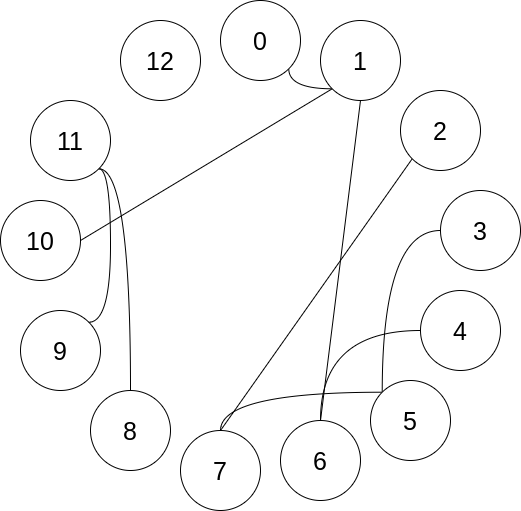
\includegraphics[width=200px]{images/7_Hashing/mophf_graph.png}
\end{figure}
If there is a cycle inside the graph we throw away the structure and recompute $h$.

Now we can build the equations:
$$
    h(abacus)= 0 \implies g(h_1(abacus)) + g(h_2(abacus)) = 0 \mod 9 \\
    \implies g(1) + g(6) = 0 \mod 9
$$
at the end we build $n$ equations in $m$ variables (the values of $g$) that can be solved in a lot of ways.
We'll solve it using the graph itself writing the solutions over the arcs in the graph: we can set $g(x)$ as the value we want for one of the nodes, and then from it we navigate the graph solving the equations:
\begin{itemize}
    \item we set $g(2) = 0$;
    \item $g(2) + g(7) = 1 \implies g(7) = 1$;
    \item $g(7) + g(5) = 2 \implies g(5) = 1$;
    \item $g(5) + g(3) = 8 \implies g(3) = 7$;
    \item of course when a path is over we start again by picking a node, setting a value for it and then again traversing the graph until all the nodes are done.
\end{itemize}
\begin{figure}[H]
    \centering
    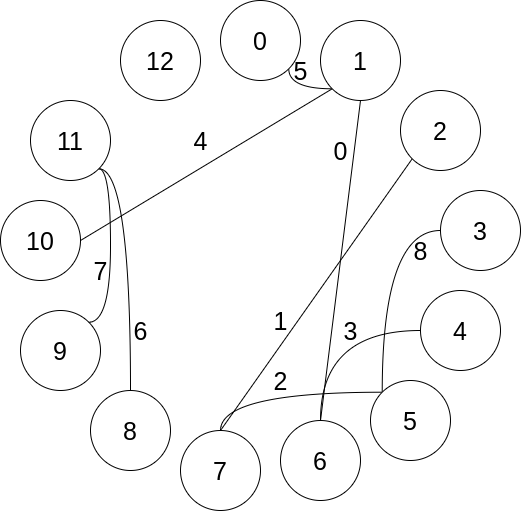
\includegraphics[width=200px]{images/7_Hashing/mophf_graph_solved.png}
\end{figure}

To build $g$ we need $O(m)$ time and $O(n)$ space, which is the table for $g$.
To store $h_1$ and $h_2$ we can use $ax + b \mod p \mod m'$ because they are universal hashes, so we can build the hash-table without storing the strings.

During the search we hash the string using $h_1$ and $h_2$, we access $g$ at those indexes and sum the results.

\section{Bloom filters}
In the context of dictionary problem a bloom filter allows us to:
\begin{itemize}
    \item $insert(k)$;
    \item $membership(k)$.
\end{itemize}
we can't delete a key!

It is a very succint data structure because it does not store the keys, as a drawbacks we can incur into \emph{false positive} errors, so a match means a \emph{maybe}.
It's called \emph{one side error} because a yes is a maybe but no is no.
Moreover we can control the error (eg make it really small)!

We need:
\begin{itemize}
    \item $r$ different universal hash function: $h_1$, $h_2$, \_, $h_r$:
    $$
        h_i : U \xrightarrow{} [m], m > n
    $$
    \item a binary array $B[0, m-1]$
\end{itemize}

\subsection{Insertion}
To insert $k$ we set:
$$
    B[h_i(k)] = 1 \forall i = 1, 2, \_, r
$$
insertion is $O(r)$ time.

\subsection{Membership}
Given a key $k$ we return:
$$
    yes \iff B[h_i(k)] = 1 \forall i = 1, 2, \_, r
$$

\subsection{Complexity}
A bloom filter occupies $m$ bits ($m = r \cdot n$ with $r \approx 30-60$) while hashing with chaining/cuckoo hashing uses $m \geq 2 c n \cdot log_2 U$ bits, so if the constant multiplied by $n$ is $<$ 60 it's more useful to go with cuckoo hashing.

In modern database $B^+$-tree is used and each level stores a bloom filter that stops tree visit if it says no, in order to prevent some I/Os.

Let's estimate $\mathbb{P}(B[j] = 0)$: we have $n$ keys and every key have to set $r$ bits, so:
$$
    \mathbb{P}(B[j] = 0) = \left( \frac{m-1}{m} \right)^{n r} = \left( 1 - \frac{1}{m} \right)^{n r} = \left( 1 - \frac{1}{m} \right)^{\frac{n r}{m} \cdot m}
$$
$$
    = \left[ \left( 1 - \frac{1}{m} \right)^m \right]^{\frac{r n}{m}} \xrightarrow{\infty} e^{-\frac{r n}{m}}
$$
so:
$$
    \mathbb{P}(B[j] = 1) = 1 - e^{- \frac{r n}{m}}
$$

NB: we are supposing that $B[a]$ is independent from $B[b]$ which is not correct but a good approximation.

Let's estimate the error:
$$
    \mathbb{P}(error) = \mathbb{P}(k \notin D \land \forall i =1, 2, \_, r B[h_i(k)] = 1)
$$
$$
    = \mathbb{P}(B[j_1] = 1 \land B[j_2] = 1 \land \_ \land B[j_r] = 1) \approx \mathbb{P}(B[j] = 1)^r = (1 - e^{-\frac{r n}{m}})^r
$$
To study the function we fix two variables and vary the last one, let's fix $m$ and $n$, we have a function in $r$.
Studying the function we can find that the minimum error is gained for:
$$ 
    r_{opt} = \frac{m}{n} ln 2
$$
which gives us the error:
$$
    \epsilon_{opt} = \left( \frac{1}{2} \right)^{r_{opt}} = (0.6...)^{\frac{m}{n}}
$$
so each bit we add decreases the error by a factor 0.6.

Eg: $m = 2n \xrightarrow{} \epsilon_{opt} = 0.38$, $m = 5n \xrightarrow{} \epsilon_{opt} = 0.09$, so an error rate of 9\%!

Of course the less the error we want, the more the hash function and the size we need, so usually we give away the minimal error and use $r = 20$ with $\epsilon = \left( 1 - e^{- \frac{20n}{m}} \right)^{20}$.

We have a lower bound: every data structure which makes an error $\epsilon$ over $n$ keys occupying space $m$ must use $m$ bits s.t.:
$$
    m \geq n \cdot log_2 \frac{1}{\epsilon}
$$
For bloom filters in particular (in optimal case):
$$
    \epsilon =2^{\frac{m}{n} ln(2)} \implies \frac{1}{\epsilon} = 2^{\frac{m}{n} ln(2)} \implies log_2 \frac{1}{\epsilon} = \frac{m}{n} ln(2)
$$
$$
    \implies m = \frac{1}{ln(2)} \cdot n \cdot log_2 \frac{1}{\epsilon}
$$
so we have a factor different from the lower bound.

\subsubsection{Example of usage}
Two machines in a p2p network wants to synchronize their knowledge, so we have two sets $A$ and $B$ and we want to compute $A \cap B$.
Let's suppose that $A$ wants to send hashes of movies: $|A| log_2 U$ bits sent, $A$ builds up $BF_A$ of size $m_A$ ($\epsilon = (0.6)^{\frac{m_A}{n_A}}$) and sends it.
So $A$ sends $m_A$ bits.
Then $B$ receives $BF_A$ and $\forall b \in B : BF_A(b) =$:
\begin{itemize}
    \item yes: $b$ maybe $\in A \cap B$: it's yes for sure for $b \in A \cap B$ and is yes for some $b \in B \cap b \notin A$ which are the errors;
    \item no: $b \notin A$, so $b \notin A \cap B$ and we download it.
\end{itemize}
So let's assume that $\epsilon = 1\%$:
$$
    \mathbb{E}[errors] = \#\text{checked elements} \cdot (0.6)^{\frac{m_A}{n_A}} \leq |B|\cdot(0.6)^{\frac{m_A}{n_A}}
$$
so we will get $\#yes = |A \cap B| + |B|\cdot(0.6)^{\frac{m_A}{n_A}}$ which is the number of correct plus the number of errors.

\subsection{Spectral bloom filter}
The spectral bloom filter allows us to:
\begin{itemize}
    \item $counting(k)$;
    \item $insertion(k)$/$increasing(k)$;
    \item $deletion(k)$/$decreasing(k)$
\end{itemize}
instead of a binary array we use an array of integers of 32 or 64 bits $C$, then we use $r$ hash functions $h_1, h_2, \_, h_r : U \xrightarrow{} [m]$.

\subsubsection{Increment}
$$
    C[h_i(k)] += 1 \forall i = 1, 2, \_, r
$$

\subsubsection{Decrement}
$$
    C[h_i(k)] -= 1 \forall i = 1, 2, \_, r
$$

\subsubsection{Counting}
$$
    min_{1 \leq i \leq r} C[h_i(k)]
$$

The probability of an error is the same as usual bloom filter:
$$
    \mathbb{P}(error) = \left( \frac{1}{2} \right)^{r_{opt}} = (0.6)^{\frac{m}{n}}
$$

